\textbf{Requirements of the power system}

 There are two boards that need to be powered on the multirotor RPAS, the Raspberry Pi, and the Zedboard. The Raspberry Pi requires
5 V, has a maximum current draw of 1 A and a typical current draw of 400 mA. The Zedboard requires 12 V, has a maximum current draw of
4 A and a typical current draw of 1 A. The power system also
needs to be light-weight to minimize the impact on the multirotor's performance. The power system also needs to provide continuous power to the computing platform for at least 10 minutes.

\textbf{The battery}

We choose to use a Lithium-ion or Lithium-polymer battery with a battery management system. In order to
power the computing system for 10 minutes the battery will need to have a capacity of 233mAh, however as that is a non-standard size and also to allow for a margin of error an 11.1V battery with a 1000mAh capacity will be used. This should provide 43 minutes of operation.

\textbf{The battery management system}

The battery management system will need to provide a number of key functions. These are:
  
  \begin{itemize}
\item Provide constant 12V and 5V outputs even as the battery voltage degrades
\item Withstand 1A of continous current in the 5V output and 4A continous current in the 12V output
\item Has a safety cutoff or warning if the battery voltage is too low.
\item Has overcurrent protection.
\item Has overvoltage protection.
\item Have reverse polarity protection
\end{itemize}
 
The battery management system should also ideally do all of the above at the highest efficiency and lowest weight and cost possible. With all of the above in mind the battery management system will consist of two DC-DC converters, a battery protection board and a battery monitor. The DC-DC converters will be a buck converter for the 5V output and a buck-boost converter for the 12V output. The battery protection board will consist of a Zener diode to provide overcurrent protection, a fuse to provide overcurrent protection, and a simple circuit to provide reverse polarity protection. Reverse polarity protection will also be provided by using connectors that cannot be connected backwards. A battery monitor will be plugged into the lipo that will alert us to the battery voltage being too low.

Lastly a seperate charger will be needed to charge the battery.

\begin{figure}\label{Overview}
\centering
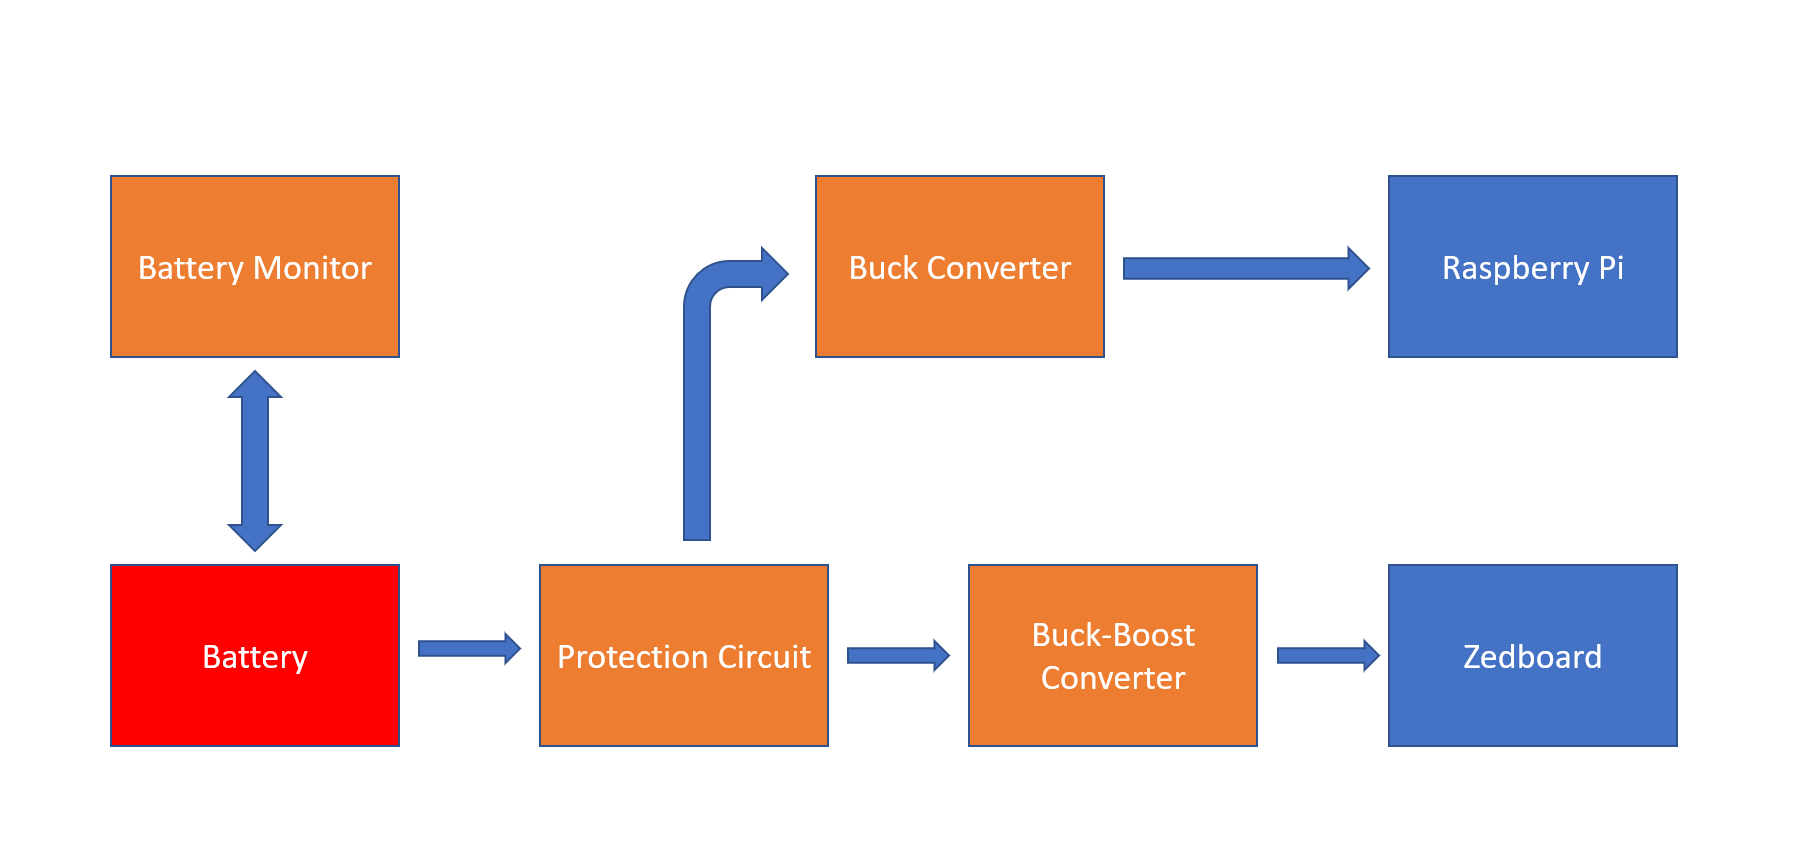
\includegraphics[width=10cm]{img/Power_Diagram.png}
\end{figure}
